\documentclass{minimal}

\usepackage{pdflscape}
\usepackage{tikz}

\usetikzlibrary{er, positioning, fit}
\tikzset{multi attribute/.style = {attribute, double distance=1.5pt}}
\tikzset{total relation/.style = {-, double, double distance=1.5pt}}

\begin{document}

\begin{landscape}
  \begin{center}
    \begin{tikzpicture}[auto,node distance=1.5cm]
      \node[entity] (film) {Film}

      child {node[attribute, right = of film] (year) {Release Year}}
      child {node[attribute, above = 1cm of year, minimum width = 1cm]
        (filmId) {\underline{ID}}}
      child {node[attribute, left = of film] (description) {Description}}
      child {node[attribute, above = 1cm of description] (title) {Title}};


        \node[relationship] (availablelanguage)
        [below right = 3cm of film, minimum size=1.5cm]
      {Available In};

      \node[entity] (language) [below right = of availablelanguage] {Language}
        [grow = down, sibling distance=3cm]
        child {node[attribute, minimum width = 1cm] {\underline{ID}}}
        child {node[attribute] {Full name}};

        \path (availablelanguage)
        edge node {m} (film)
        edge node {n}(language);



        \node[relationship] (relFilmMedia) [below = 3cm of film] {Supports};

        \node[entity] [below = of relFilmMedia] (media) {Media Type}
        [grow = down, sibling distance = 3cm]
        child {node[attribute, minimum width = 1cm] {\underline{ID}}}
        child {node[attribute] {Name}};

        \path (relFilmMedia)
        edge node {m} (film)
        edge node {1} (media);



        \node[relationship] (relFilmGenre) [below left = 3cm of film]
        {Classified as};

        \node[entity] [below left = of relFilmGenre] (genre) {Genre}
        [grow = down, sibling distance = 3cm]
        child {node[attribute, minimum width = 1cm] {\underline{ID}}}
        child {node[attribute] {Name}};

        \path (relFilmGenre)
        edge node {m} (film)
        edge node {1} (genre);


        \node[relationship] (relFilmActor) [above = of film, minimum size=1.5cm]
        {Credit}
        child[grow=left, level distance=2cm] {node[attribute] {Role}};

        \node[rectangle, draw=black, fit=(relFilmActor), inner sep=0em]
        (relFilmActorSq) {};

        \node[entity] (actor) [above = of relFilmActor] {Actor}
        [grow = up, sibling distance=3cm]
        child {node[attribute, minimum width = 1cm] {\underline{ID}}}
        child {node[attribute] {Full Name}};

        \path (relFilmActor)
        edge node {m} (film)
        edge[total relation] node {n} (actor);
    \end{tikzpicture}

  \pagebreak

  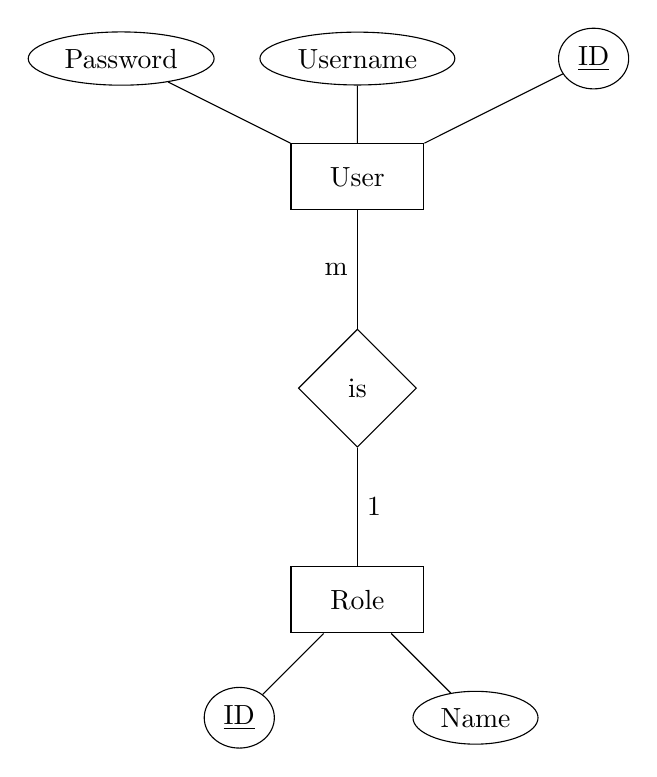
\begin{tikzpicture}[auto,node distance=1.5cm, sibling distance = 3cm]
    \node[entity] (user) {User}
    [grow = up]
    child {node[attribute] {\underline{ID}}}
    child {node[attribute] {Username}}
    child {node[attribute] {Password}};

    \node[relationship] (relUserRole) [below = of user, minimum width = 1.5cm,
    minimum height = 1.5cm] {is};

    \node[entity] (role) [below = of relUserRole] {Role}
    [grow = down]
    child {node[attribute] {\underline{ID}}}
    child {node[attribute] {Name}};

    \path (relUserRole)
    edge node {m} (user)
    edge node {1} (role);
  \end{tikzpicture}

  \end{center}
\end{landscape}

\end{document}
